In this chapter, the most important libraries used while implementing our application, will be described.
Besides libraries, the undo algorithm will be also described at the end of this chapter.

It is advantageous to use libraries when programming, because some parts that are needed to be implemented in the application have already been implemented by someone else and may be available in the form of libraries.
Using these solutions not only saves time, but it also prevents creating bugs while trying to implement these parts of code.

\section{Room}
Room is a persistence library that was decided to be used in our application in \autoref{subsec:daoandnetwork}.

Room makes it easier to work with an application's internal database.
For each entity stored in the database, an entity class is defined, which is just a standard Kotlin class with some annotations.
The simplest entity class looks as follows.
The whole class is annotated with \verb|@Entity| and primary key is annotated with \verb|@PrimaryKey|.
In case there is a need for multiple primary keys, they can be listed in the \verb|@Entity| annotation.
DAO classes are annotated with \verb|@Dao| and are used to store and load objects to and from the database.
Creating DAO classes is done by declaring abstract methods with annotations, optionally accompanied by SQL syntax.
Those methods are being implemented by Room.
Entities, lists of entities or LiveData instances of either of those can be returned by the DAO's methods.

\section{LiveData}
LiveData is an observable data structure, that was decided to be used in our application in \autoref{subsec:observable}

View components can observe this observable structure by registering instances of \verb|Observer|.
When registering an \verb|Observer|, the view have to pass an instance of it's lifecycle, so the LiveData instance can detect when to remove this \verb|Observer|, so no memory leaks are created and so the performance stays the same.
Previously mentioned library Room can also return LiveData instances, so observers can react to database changes directly, without any other unnecessary code.

\section{Retrofit}
Retrofit is a HTTP library specialized for implementing REST API clients, that has been decided to be used in our application in \autoref{subsec:daoandnetwork}.

An abstract method is declared for each API call, complemented with an annotation with HTTP request details.
Retrofit also uses the OkHttp \cite{okhttp} library, where the basic authentication can be arranged.

\section{Coroutines}
Coroutines are Kotlin's way to improve multithreaded programming.
Compared to Java, Kotlin introduces a new keyword \verb|suspend| that can be written in front of methods.
Methods with the \verb|suspend| keyword can not be called the normal way, but can be called from other \verb|suspend| methods or launched via higher order methods of \verb|CoroutineScope|.
Although \verb|suspend| is a Kotlin's keyword, dependency for a library is needed in order to work with coroutines and that is why Coroutines are described here, between libraries.

\section{Scheduling of asynchronous tasks}
Service is a part of an application that can run in background and can be started even when the application is not running.
Our application needs services for checking execution statuses.
Scheduling services across multiple Android versions can be tricky, so using a library for his purpose is a good option.
Popular solutions for scheduling services are Android-Job \cite{androidjob} and WorkManager \cite{workmanager}.
The readme file of Android-Job states that it is deprecated and that WorkManager should be used instead \cite{androidjob}.
Because of that, WorkManager will be used for scheduling services.

\section{QR code scanner}
There is a need to implement a QR code scanner, because of \autoref{subsec:qrcode}.
ZXing library \cite{zxing}, Mobile Vision \cite{vision}, or Varvet's QR code scanner \cite{varvet} can be used.

When using the ZXing library, a third party application needs to be downloaded to the phone, which can be unpleasant.
Mobile Vision is a new library from Google that allows scanning QR codes without the need of a third party application.
Varvet's QR code scanner is a library based on Google's Mobile Vision.
For the purpose of reading QR codes, the Varvet's QR code scanner is easier to implement than the Mobile Vision library.

Varvet's QR code scanner will be used for scanning QR codes in our application.

\section{Draggable Views}
Pipeline's components should be freely movable across the canvas while editing the pipeline.
That can be achieved by making some regular view (button or image) movable.
This is often achieved by a lot of unnecessary code and that is why a library will be used for this purpose.

The only library suited for this purpose, that has been found, is DraggableView by hyuwah \cite{draggable}.
It allows programmers to turn any view into a draggable view, which means it can be moved with a finger.

\section{Undo operations}
In \autoref{chap:requirementsengineering} are some undo options in planning.
The user should be able to undo the deletions of pipelines and executions.
It can not be done just by scheduling the sending of the delete request.
The application will create and store a mark for every deleted item alongside with scheduling the delete request (see \autoref{fig:undoDelete}).
Because of that, when the application is killed for any reason before the delete request is sent, the application can check all of those marks at the application launch and send the delete requests then (see \autoref{fig:undoDbClean}).
Marks can also be used for filtering pipelines and executions that will be shown to the user.
If the user undo the deletion, the mark is deleted and the scheduling of the delete request is cancelled (see \autoref{fig:undoUndo}).

\begin{figure}\centering
    \begin{minipage}[b]{0.45\textwidth}
    	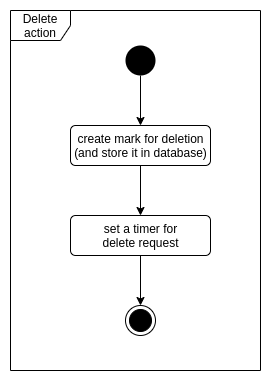
\includegraphics[width=\textwidth]{pics/undo/delete_action.png}
    	\caption[Delete action]{Delete action}\label{fig:undoDelete}
    \end{minipage}
    \begin{minipage}[b]{0.45\textwidth}
    	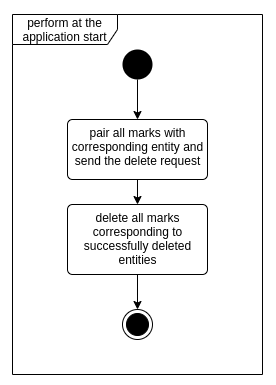
\includegraphics[width=\textwidth]{pics/undo/db_clean.png}
    	\caption[Finish interrupted delete actions]{Finish interrupted delete actions}\label{fig:undoDbClean}
    \end{minipage}
    \begin{minipage}[b]{0.45\textwidth}
    	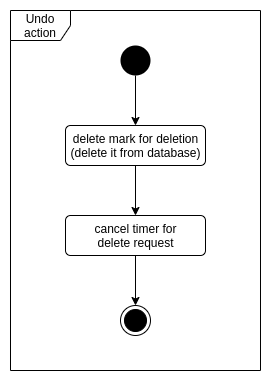
\includegraphics[width=\textwidth]{pics/undo/undo_action.png}
    	\caption[Undo action]{Undo action}\label{fig:undoUndo}
    \end{minipage}
\end{figure}